\documentclass[11pt]{article}

\usepackage[margin=1in]{geometry}
\usepackage{times}
\usepackage{graphicx}
\usepackage{amsmath, amssymb}
\usepackage{booktabs}
\usepackage{array}
\usepackage{algorithm}
\usepackage{algorithmic}
\usepackage{multirow}
\usepackage{xcolor}
\usepackage{hyperref}
\usepackage{caption}
\usepackage{placeins}
\usepackage{float}
\usepackage{indentfirst}
\usepackage[numbers]{natbib}

\hypersetup{
    colorlinks=true,
    linkcolor=blue,
    citecolor=blue,
    urlcolor=blue
}

\setlength{\parindent}{1.5em}
\setlength{\parskip}{0pt}

\title{\textbf{PetMIM: Structure-Aware Masked Image Modeling for Pet Image Segmentation}}

\author{
Chenxuan Ning \quad Dongxu Wang \quad Haoran Zhang\\
Beijing University of Posts and Telecommunications
}

\date{June 2026}

\begin{document}

\maketitle

\begin{abstract}
\hspace{\parindent}Pet image segmentation is a fine-grained foreground segmentation task that requires accurate localization of object regions and boundary details around fur, ears, legs, and low-contrast foreground-background transitions. Supervised encoder-decoder networks can learn the dominant pet body region, but they may not explicitly encourage the encoder to focus on local structures that are important for boundary-sensitive segmentation. This paper presents PetMIM, a structure-aware masked image modeling pretraining strategy for pet foreground segmentation. PetMIM estimates a patch-level structure score from edge response, texture variation, and low color contrast, and uses the score to guide a mixed masking strategy. The learned encoder is then transferred to a downstream ResNet18-U-Net segmentation model. Experiments on Oxford-IIIT Pet show that PetMIM improves global overlap, spatial distance, boundary-sensitive metrics, and hard-case performance compared with scratch training and random MIM pretraining. These results suggest that task-aware masking can make self-supervised pretraining more suitable for pet boundary segmentation.
\end{abstract}

\textbf{Keywords:} pet segmentation; masked image modeling; self-supervised pretraining; boundary-sensitive evaluation; ResNet18-U-Net.

\section{Introduction}

Image segmentation is a fundamental dense prediction problem in computer vision. Unlike image classification, which assigns a single label to an image, segmentation requires assigning labels to individual pixels and therefore depends on both semantic recognition and spatial localization. In natural images, foreground object segmentation is especially challenging when the object boundary is fuzzy, when the object appearance is similar to the background, or when fine local structures determine the exact contour. Pet foreground segmentation is a representative example of this setting. Cats and dogs often contain thin legs, ears, tails, and fur-like boundaries, and their appearance may be visually close to carpets, floors, shadows, or indoor backgrounds.

The Oxford-IIIT Pet dataset provides pixel-level trimap annotations for cats and dogs, making it a suitable benchmark for studying pet foreground segmentation under boundary-sensitive evaluation~\cite{parkhi2012cats}. Broader natural-image segmentation benchmarks, such as PASCAL VOC~\cite{everingham2010pascal} and COCO~\cite{lin2014microsoft}, also include animal categories and demonstrate that animal segmentation is a common real-world dense prediction problem. Most segmentation pipelines focus on improving the supervised segmentation architecture, for example through fully convolutional prediction~\cite{long2015fully}, encoder-decoder structures such as U-Net~\cite{ronneberger2015unet}, atrous convolution and decoder refinement~\cite{chen2018encoder}, or Transformer-based segmentation backbones~\cite{xie2021segformer}. These methods are powerful, but they still rely on supervised pixel annotations to shape the representation used by the encoder.

Self-supervised pretraining provides another route for improving segmentation. Instead of changing the downstream model, it learns transferable visual representations from images before supervised fine-tuning. Contrastive and non-contrastive self-supervised methods such as SimCLR~\cite{chen2020simclr}, MoCo~\cite{he2020moco}, BYOL~\cite{grill2020byol}, and SimSiam~\cite{chen2021simsiam} have shown that visual encoders can learn useful representations without labels. Masked image modeling (MIM) is particularly relevant to segmentation because it trains a model to reconstruct missing image regions from visible context. BEiT~\cite{bao2022beit}, MAE~\cite{he2022masked}, SimMIM~\cite{xie2022simmim}, MaskFeat~\cite{wei2022masked}, and later CNN-compatible MIM methods such as SparK~\cite{tian2023spark} demonstrate the effectiveness of reconstruction-based pretraining.

However, the masking policy in standard MIM is usually random. Random masking is general, but it is not aware of the downstream segmentation task. For pet segmentation, patches near fur boundaries, texture transitions, and low-contrast foreground-background regions are more likely to affect mask quality than homogeneous interior patches. This observation is related to recent task-aware masking ideas. For example, OrgMIM shows that structural priors and reconstruction difficulty can guide MIM masking for organelle segmentation in volume electron microscopy~\cite{zhang2026orgmim}. Although the domain is different, the key principle is useful: a segmentation-oriented pretraining task should encourage the model to reconstruct structures that matter for downstream masks.

This paper proposes PetMIM, a lightweight structure-aware MIM strategy for pet image segmentation. PetMIM computes a patch-level score using only the input RGB image, combining edge response, local texture variation, and low color contrast. It then masks a mixture of high-score patches and random patches. The method keeps the downstream segmentation architecture fixed and changes only the pretraining strategy, making the comparison against scratch training and RandomMIM direct. The method is designed to answer a focused question: can a simple task-aware masking rule help MIM learn features that are more useful for pet foreground segmentation?

In summary, PetMIM contributes a structure score for pet-oriented patch selection, a mixed structure-aware masking strategy for MIM pretraining, and an evaluation protocol that includes global overlap, spatial distance, Boundary F1, and trimap-region metrics. The results show consistent improvements on the main Oxford-IIIT Pet setting and stronger performance on predefined hard-boundary and low-contrast subsets.

\section{Related Work}

\textbf{Natural-image and pet segmentation.} Fully convolutional networks formulate semantic segmentation as end-to-end dense prediction~\cite{long2015fully}. U-Net introduces an encoder-decoder architecture with skip connections, allowing low-level spatial details to be fused with high-level semantic features~\cite{ronneberger2015unet}. DeepLabV3+ improves semantic segmentation through atrous separable convolution and decoder refinement~\cite{chen2018encoder}, while SegFormer demonstrates the effectiveness of Transformer-style encoders for dense prediction~\cite{xie2021segformer}. Boundary-aware methods are also related to pet foreground segmentation. BASNet explicitly models object boundaries for salient object detection~\cite{qin2019basnet}, Boundary Loss optimizes segmentation from a contour perspective~\cite{kervadec2019boundary}, and PointRend refines uncertain points to obtain sharper segmentation boundaries~\cite{kirillov2020pointrend}. These methods show that dense prediction performance depends not only on semantic recognition but also on spatial and boundary accuracy. PetMIM differs from these supervised segmentation methods because it does not introduce a new segmentation decoder or boundary loss. Instead, it improves the encoder through structure-aware pretraining while keeping the downstream segmentation model fixed.

\textbf{Self-supervised visual pretraining.} Self-supervised learning aims to learn visual representations from unlabeled images. Contrastive learning methods such as SimCLR~\cite{chen2020simclr} and MoCo~\cite{he2020moco} learn invariance between augmented views, while BYOL~\cite{grill2020byol} and SimSiam~\cite{chen2021simsiam} reduce the need for negative pairs. These approaches are general-purpose pretraining methods and have influenced many downstream vision tasks. For segmentation, however, local spatial details and boundary structures are especially important. MIM is therefore attractive because its reconstruction task preserves the spatial nature of the image. BEiT predicts visual tokens for masked patches~\cite{bao2022beit}; MAE reconstructs masked image patches with an asymmetric encoder-decoder design~\cite{he2022masked}; SimMIM shows that simple pixel reconstruction can be effective~\cite{xie2022simmim}; and MaskFeat reconstructs hand-crafted features rather than raw pixels~\cite{wei2022masked}. CNN-oriented MIM methods such as SparK further extend masked reconstruction beyond Vision Transformers~\cite{tian2023spark}. PetMIM follows the MIM paradigm but changes the masking policy from random selection to structure-aware mixed selection.

\textbf{Task-aware masking for segmentation.} The quality of a MIM pretraining task depends strongly on what is masked. Random masking can provide broad coverage, but it may waste pretraining effort on easy or less informative regions. Recent work has explored more targeted masking strategies. OrgMIM, for example, uses organelle membrane priors and reconstruction feedback to generate masks that emphasize biologically meaningful structures for EM organelle segmentation~\cite{zhang2026orgmim}. PetMIM adapts this general idea to natural pet images with a simpler and lighter design. Since pet images do not provide membrane priors or 3D volumes, PetMIM instead uses RGB-derived edge, texture, and low-contrast cues to identify patches that are likely to influence foreground segmentation.


\begin{figure}[H]
    \centering
    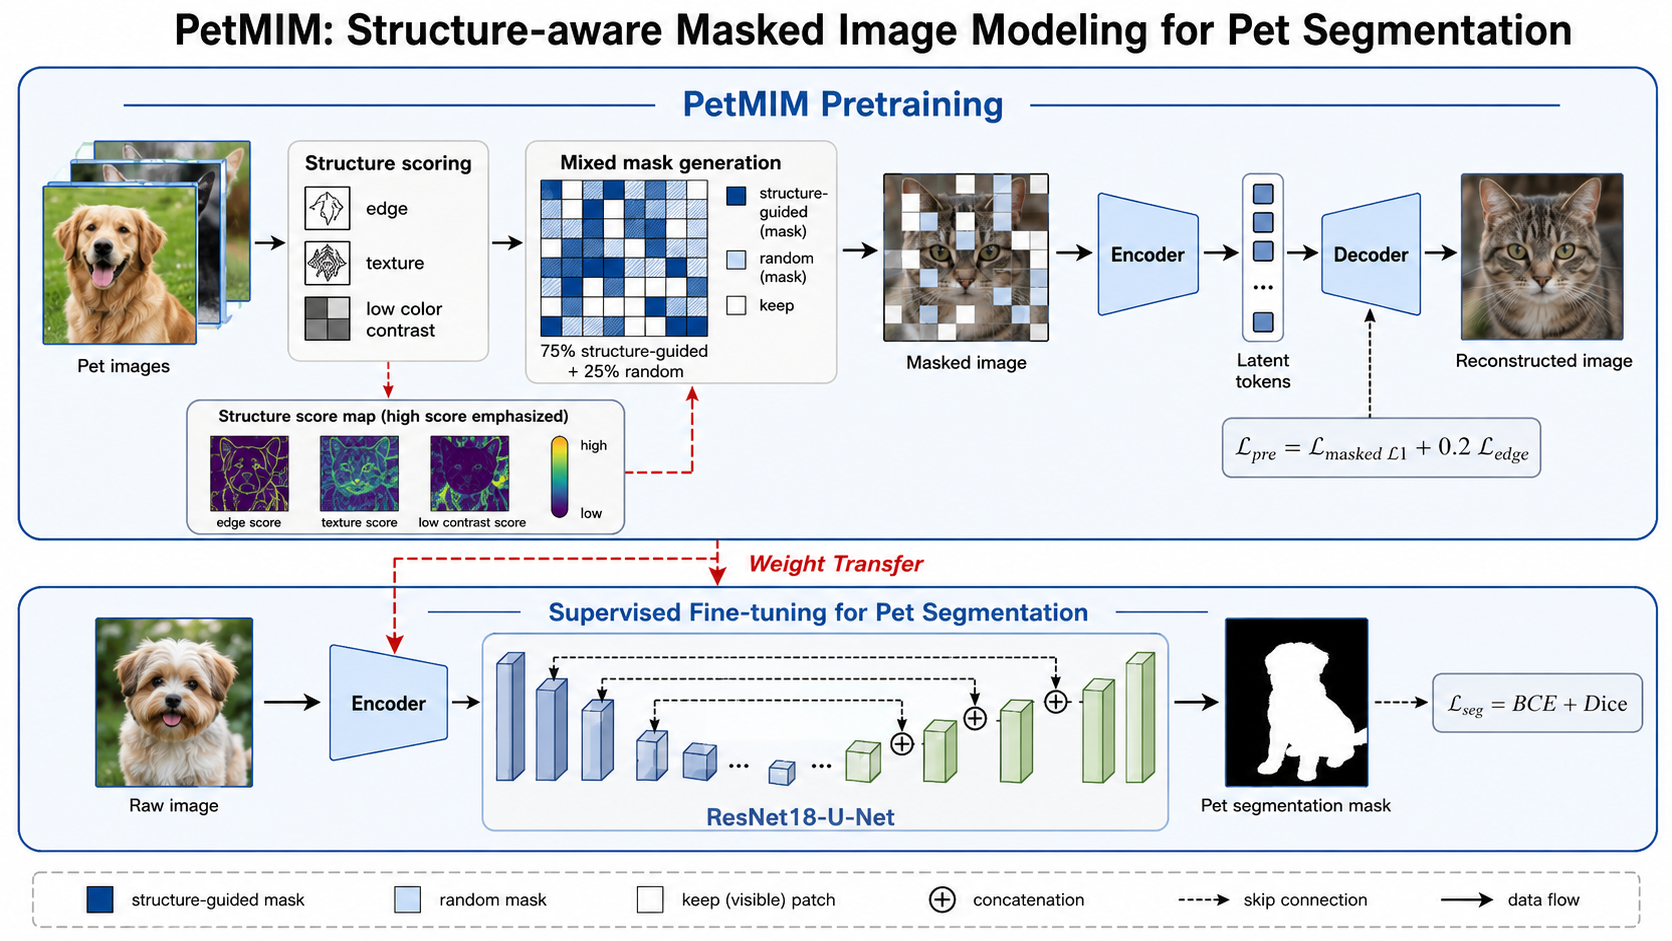
\includegraphics[width=0.98\linewidth]{figures/petmim_pipeline_overview_for_segmentation.png}
    \caption{Overall pipeline of PetMIM. The upper branch performs structure-aware masked image modeling pretraining, and the lower branch transfers the pretrained encoder to ResNet18-U-Net for supervised pet segmentation.}
    \label{fig:pipeline}
\end{figure}

\section{Method}

Figure~\ref{fig:pipeline} shows the overall PetMIM pipeline. The method contains a self-supervised pretraining stage and a supervised fine-tuning stage. During pretraining, an input pet image is divided into patches, each patch is assigned a structure score, and a mixed mask is generated from high-score and random patches. The masked image is reconstructed by an encoder-decoder model. During fine-tuning, the reconstruction decoder is discarded, and the pretrained encoder is transferred into a ResNet18-U-Net segmentation network.


\subsection{Structure-Aware MIM Pretraining}

Let an image be resized to $224 \times 224$ and divided into $16 \times 16$ patches. This gives a $14 \times 14$ patch grid with 196 patches. For each patch $p$, PetMIM defines the final structure score as
\begin{equation}
S(p) = (0.6E(p) + 0.4T(p)) \cdot (0.5 + 0.5C_{\mathrm{low}}(p)),
\label{eq:score}
\end{equation}
where $E(p)$ is an edge score, $T(p)$ is a texture score, and $C_{\mathrm{low}}(p)$ is a low-color-contrast score. This score is not a semantic foreground probability. It is a pretraining guidance signal that identifies patches where segmentation is likely to be sensitive: object contours, fur-like local variation, and visually ambiguous foreground-background transitions.

The edge score is the average gradient magnitude in the patch:
\begin{equation}
E(p)=
\mathrm{Norm}\left(
\frac{1}{|p|}
\sum_{(i,j)\in p}
|\nabla I_{\mathrm{gray}}(i,j)|
\right).
\label{eq:edge}
\end{equation}
Edges are used because pet masks are largely determined by contour locations. Errors around ears, legs, tails, and fur boundaries often correspond to small spatial shifts of high-gradient regions. By assigning higher scores to patches with stronger gradients, PetMIM increases the probability that the encoder must reconstruct boundary-related evidence during pretraining.

The texture score is the standard deviation of grayscale intensities in the patch:
\begin{equation}
T(p)=
\mathrm{Norm}\left(
\mathrm{Std}_{(i,j)\in p}(I_{\mathrm{gray}}(i,j))
\right).
\label{eq:texture}
\end{equation}
Texture is included because pet boundaries are not always represented by a single clean edge. Fur regions may contain repeated local variations, and the transition between the animal body and the background may be distributed across several patches. A texture term complements the edge term by emphasizing locally informative but less sharply defined regions.

The low-color-contrast score is defined from the difference between the mean RGB color of patch $p$ and its neighboring patches $\mathcal{N}(p)$:
\begin{equation}
C_{\mathrm{low}}(p)=
1-
\mathrm{Norm}\left(
\frac{1}{|\mathcal{N}(p)|}
\sum_{q\in \mathcal{N}(p)}
\|\mu_{\mathrm{RGB}}(p)-\mu_{\mathrm{RGB}}(q)\|_2
\right).
\label{eq:contrast}
\end{equation}
This term gives higher values to patches whose local colors are similar to their neighbors. Such areas are difficult for foreground segmentation because pet and background appearances can be close, for example light fur against a light floor or dark fur against a shadowed background. In Eq.~\eqref{eq:score}, $C_{\mathrm{low}}(p)$ is used as a multiplicative factor rather than an independent additive term. This design allows low contrast to increase the importance of patches that already contain edge or texture evidence, instead of highlighting flat and uninformative regions.

Here $\mathrm{Norm}(\cdot)$ denotes robust percentile normalization:
\begin{equation}
\mathrm{Norm}(x)=
\mathrm{clip}\left(
\frac{x-P_1(x)}{P_{99}(x)-P_1(x)+\epsilon},
0,1
\right),
\label{eq:norm}
\end{equation}
where $P_1$ and $P_{99}$ are the 1st and 99th percentiles. This normalization keeps the three score components on a comparable scale and reduces the effect of isolated noise or extreme local gradients.

RandomMIM uniformly samples masked patches. PetMIM instead masks a mixture of structure-guided and random patches. Let $N$ be the number of patches and $r$ be the total masking ratio. We use $r=0.25$, so approximately 49 of the 196 patches are masked. Among them, 75\% are selected from the highest-score structure patches and 25\% are sampled randomly from the remaining patches. The masking process is summarized in Algorithm~\ref{alg:mask}, and the score-to-mask process is visualized in Figure~\ref{fig:masking}.

\begin{algorithm}[H]
\caption{PetMIM mixed masking.}
\label{alg:mask}
\begin{algorithmic}[1]
\STATE \textbf{Input:} image $I$, patch size 16, mask ratio $r=0.25$, structure fraction $\alpha=0.75$
\STATE Compute patch structure score $S(p)$ for all patches using Eq.~\eqref{eq:score}
\STATE $k \leftarrow \mathrm{round}(rN)$, $k_s \leftarrow \mathrm{round}(\alpha k)$, $k_r \leftarrow k-k_s$
\STATE Select $k_s$ patches with the highest structure scores
\STATE Randomly sample $k_r$ patches from the remaining patches
\STATE Fill selected patches with a fixed gray value $[0.5,0.5,0.5]$
\STATE \textbf{Return:} masked image, original image, binary mask
\end{algorithmic}
\end{algorithm}

\begin{figure}[H]
    \centering
    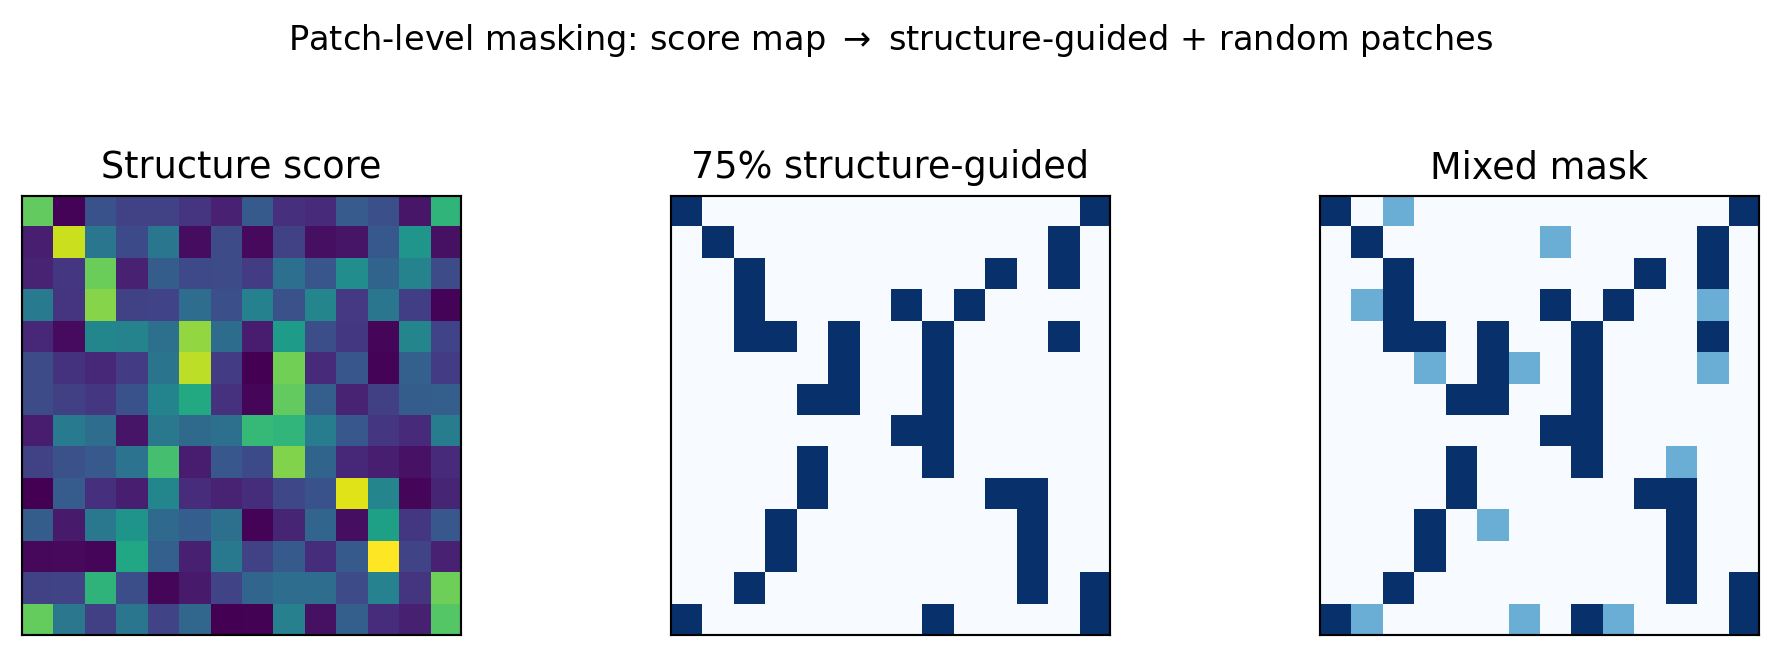
\includegraphics[width=0.92\linewidth]{figures/masking_illustration.png}
    \caption{Illustration of PetMIM masking. The structure score map highlights informative patches, 75\% of masked patches are selected from high-score regions, and the final mixed mask adds random patches to preserve diversity.}
    \label{fig:masking}
\end{figure}

The pretraining model consists of a ResNet18 encoder~\cite{he2016deep} and a lightweight reconstruction decoder. Let $X$ be the original RGB image and $\hat{X}$ be the reconstructed image. The reconstruction objective is applied only on masked pixels:
\begin{equation}
\mathcal{L}_{\mathrm{masked\_L1}}
=
|\hat{X}-X|_{\mathrm{masked}}.
\label{eq:l1}
\end{equation}
This masked L1 term forces the encoder to infer missing appearance information from visible context. Since the input mask is generated at the patch level, the model cannot solve the task by copying local pixels; it must use surrounding color, shape, and texture cues.

Plain RGB reconstruction may favor smooth color recovery and may not sufficiently preserve local boundaries. Therefore, we add an edge reconstruction term computed from gradient magnitude:
\begin{equation}
\mathcal{L}_{\mathrm{masked\_edge}}
=
\left|
|\nabla \hat{X}| - |\nabla X|
\right|_{\mathrm{masked}}.
\label{eq:edge_loss}
\end{equation}
The edge term is consistent with the downstream segmentation goal: a good pet mask depends not only on region appearance but also on the position of object contours. Penalizing differences between reconstructed and original gradient magnitudes encourages the pretrained encoder to retain boundary-sensitive features.

The total pretraining loss is
\begin{equation}
\mathcal{L}_{\mathrm{pretrain}}
=
\mathcal{L}_{\mathrm{masked\_L1}}
+
0.2\mathcal{L}_{\mathrm{masked\_edge}}.
\label{eq:pretrain_loss}
\end{equation}
The coefficient 0.2 keeps the edge term as an auxiliary constraint rather than allowing it to dominate RGB reconstruction. Importantly, the pretraining stage does not use segmentation masks. It only uses original RGB images, so the learned encoder can be transferred to the downstream segmentation model without changing the supervised training protocol.

\subsection{Downstream Pet Segmentation}

After pretraining, the reconstruction decoder is discarded. The pretrained ResNet18 encoder is loaded into a ResNet18-U-Net segmentation model. The decoder follows the U-Net-style upsampling design with skip connections, so shallow encoder features can help recover spatial details during mask prediction. The segmentation model is trained with
\begin{equation}
\mathcal{L}_{\mathrm{seg}}
=
\mathcal{L}_{\mathrm{BCEWithLogits}}
+
\mathcal{L}_{\mathrm{Dice}}.
\label{eq:seg_loss}
\end{equation}
The BCEWithLogits term provides pixel-wise supervision and stabilizes foreground-background classification. The Dice term directly optimizes region overlap and is useful when foreground and background occupy different proportions of the image. Combining the two terms gives stable pixel-level learning while still encouraging the predicted pet region to match the target mask globally.

All compared methods use the same downstream model, optimizer, preprocessing, and checkpoint selection rule. Therefore, the comparison isolates the effect of encoder initialization and masking strategy.

\section{Experiments}

\subsection{Dataset and Settings}

The main experiment uses the Oxford-IIIT Pet dataset~\cite{parkhi2012cats} through the HuggingFace dataset interface. The split contains 2567 training images, 701 validation images, and 403 test images. The trimap annotation is converted to a binary pet foreground mask; foreground and ambiguous trimap pixels are treated as foreground in the implementation. Images are resized to $224 \times 224$.

Three methods are compared:
\begin{itemize}
    \item \textbf{Scratch:} ResNet18-U-Net trained from scratch.
    \item \textbf{RandomMIM:} ResNet18 encoder pretrained with random MIM and then fine-tuned.
    \item \textbf{PetMIM:} ResNet18 encoder pretrained with the proposed structure-aware mixed MIM and then fine-tuned.
\end{itemize}

The implementation uses PyTorch 2.3.0 and torchvision 0.18.0 on an NVIDIA RTX 4090 GPU. The segmentation model is selected by the best validation Dice and evaluated once on the test set. The reported metrics include Dice, IoU, Average Distance (AD), Boundary F1 at 2 and 3 pixels, and trimap Dice/IoU with 3- and 5-pixel boundary bands.


\subsection{Main Results on Oxford-IIIT Pet}

Table~\ref{tab:main_results} shows the main test results. PetMIM obtains the best performance across all metrics. Compared with RandomMIM, PetMIM improves Dice by 0.0270 and IoU by 0.0290. It also reduces AD from 6.1616 to 4.2096, which is a relative reduction of about 31.7\%. The boundary-sensitive metrics also improve: Boundary F1@2 increases from 0.2846 to 0.2930, Boundary F1@3 from 0.3539 to 0.3646, and trimap IoU@5 from 0.4768 to 0.4887.

These results suggest that MIM pretraining is useful, since RandomMIM improves most overlap and boundary metrics over Scratch. More importantly, the additional improvement of PetMIM over RandomMIM indicates that the masking location is critical for segmentation-oriented pretraining.

\subsection{Hard-Case Analysis}

To analyze where PetMIM is most effective, three predefined hard-case subsets are constructed from the Oxford-IIIT Pet test split. The subsets are selected from image and ground-truth statistics, not from model performance. The hard-boundary subset contains the top 30\% images by boundary complexity; the low-contrast subset contains the top 30\% images with lowest foreground-background color contrast; and the high-texture subset contains the top 30\% images with highest boundary-region texture.

Table~\ref{tab:hard_cases} shows the results. PetMIM is best on all metrics for the hard-boundary and low-contrast subsets. On high-texture images, PetMIM achieves the best Dice, IoU, AD, and Boundary F1, while RandomMIM is slightly stronger on trimap overlap. This supports the design motivation of PetMIM: structure-aware pretraining is especially beneficial in cases where segmentation errors are dominated by complex boundaries and ambiguous foreground-background transitions.

\begin{table}[t]
\centering
\caption{Main results on Oxford-IIIT Pet. Higher is better for all metrics except AD.}
\label{tab:main_results}
\resizebox{\linewidth}{!}{
\begin{tabular}{lccccccccc}
\toprule
Method & Dice $\uparrow$ & IoU $\uparrow$ & AD $\downarrow$ & B-F1@2 $\uparrow$ & B-F1@3 $\uparrow$ & Tri-D@3 $\uparrow$ & Tri-I@3 $\uparrow$ & Tri-D@5 $\uparrow$ & Tri-I@5 $\uparrow$ \\
\midrule
Scratch & 0.751178 & 0.628696 & 5.687908 & 0.265837 & 0.332979 & 0.566416 & 0.416062 & 0.595845 & 0.446383 \\
RandomMIM & 0.757735 & 0.637988 & 6.161598 & 0.284580 & 0.353861 & 0.600003 & 0.445835 & 0.629264 & 0.476812 \\
\textbf{PetMIM} & \textbf{0.784777} & \textbf{0.666954} & \textbf{4.209564} & \textbf{0.293045} & \textbf{0.364595} & \textbf{0.613635} & \textbf{0.457517} & \textbf{0.642657} & \textbf{0.488665} \\
\bottomrule
\end{tabular}
}
\end{table}


\begin{table}[t]
\centering
\caption{Hard-case analysis on Oxford-IIIT Pet test images. Subsets are selected by image and ground-truth statistics before model evaluation.}
\label{tab:hard_cases}
\resizebox{\linewidth}{!}{
\begin{tabular}{llccccccccc}
\toprule
Subset & Method & Dice $\uparrow$ & IoU $\uparrow$ & AD $\downarrow$ & B-F1@2 $\uparrow$ & B-F1@3 $\uparrow$ & Tri-D@3 $\uparrow$ & Tri-I@3 $\uparrow$ & Tri-D@5 $\uparrow$ & Tri-I@5 $\uparrow$\\
\midrule
Hard-boundary & Scratch & 0.749547 & 0.620202 & 3.916755 & 0.270134 & 0.343249 & 0.611850 & 0.454252 & 0.640357 & 0.485316 \\
Hard-boundary & RandomMIM & 0.754394 & 0.622963 & 3.976004 & 0.278133 & 0.351495 & 0.631847 & 0.472891 & 0.659431 & 0.502735 \\
Hard-boundary & \textbf{PetMIM} & \textbf{0.762889} & \textbf{0.631835} & \textbf{3.611625} & \textbf{0.283966} & \textbf{0.357759} & \textbf{0.642410} & \textbf{0.482585} & \textbf{0.668170} & \textbf{0.511069} \\
\midrule
Low-contrast & Scratch & 0.717074 & 0.586858 & 4.960664 & 0.229308 & 0.289867 & 0.556327 & 0.405711 & 0.580120 & 0.429930 \\
Low-contrast & RandomMIM & 0.722389 & 0.593131 & 6.062933 & 0.239208 & 0.299372 & 0.587879 & 0.433357 & 0.612398 & 0.458122 \\
Low-contrast & \textbf{PetMIM} & \textbf{0.754648} & \textbf{0.623292} & \textbf{4.040161} & \textbf{0.251172} & \textbf{0.315238} & \textbf{0.611653} & \textbf{0.451961} & \textbf{0.634943} & \textbf{0.476010} \\
\midrule
High-texture & Scratch & 0.761113 & 0.643687 & 6.330240 & 0.290183 & 0.365495 & 0.628056 & 0.471909 & 0.654624 & 0.501622 \\
High-texture & RandomMIM & 0.754927 & 0.635336 & 6.760349 & 0.295693 & 0.372211 & \textbf{0.641609} & \textbf{0.486251} & \textbf{0.666321} & \textbf{0.513940} \\
High-texture & \textbf{PetMIM} & \textbf{0.766289} & \textbf{0.647925} & \textbf{6.299194} & \textbf{0.304053} & \textbf{0.380847} & 0.635979 & 0.479964 & 0.663069 & 0.510587 \\
\bottomrule
\end{tabular}
}
\end{table}

\subsection{Qualitative Visualization}

Figure~\ref{fig:qualitative} shows qualitative comparisons between RandomMIM and PetMIM on selected Oxford-IIIT Pet test cases. Each example contains the original image, the ground-truth mask with its trimap band, and the trimap overlays produced by RandomMIM and PetMIM. Red denotes the ground-truth trimap region, blue denotes the predicted trimap region, and purple denotes their overlap.

The selected cases cover different pet appearances, including a close-up cat, a long-haired cat, and a low-contrast spotted cat. In these examples, PetMIM produces boundary bands that are more consistent with the ground-truth trimap than RandomMIM. This visual evidence is consistent with the quantitative improvements in Boundary F1 and trimap-region metrics reported in Tables~\ref{tab:main_results} and~\ref{tab:hard_cases}.

\begin{figure}[p]
    \centering
    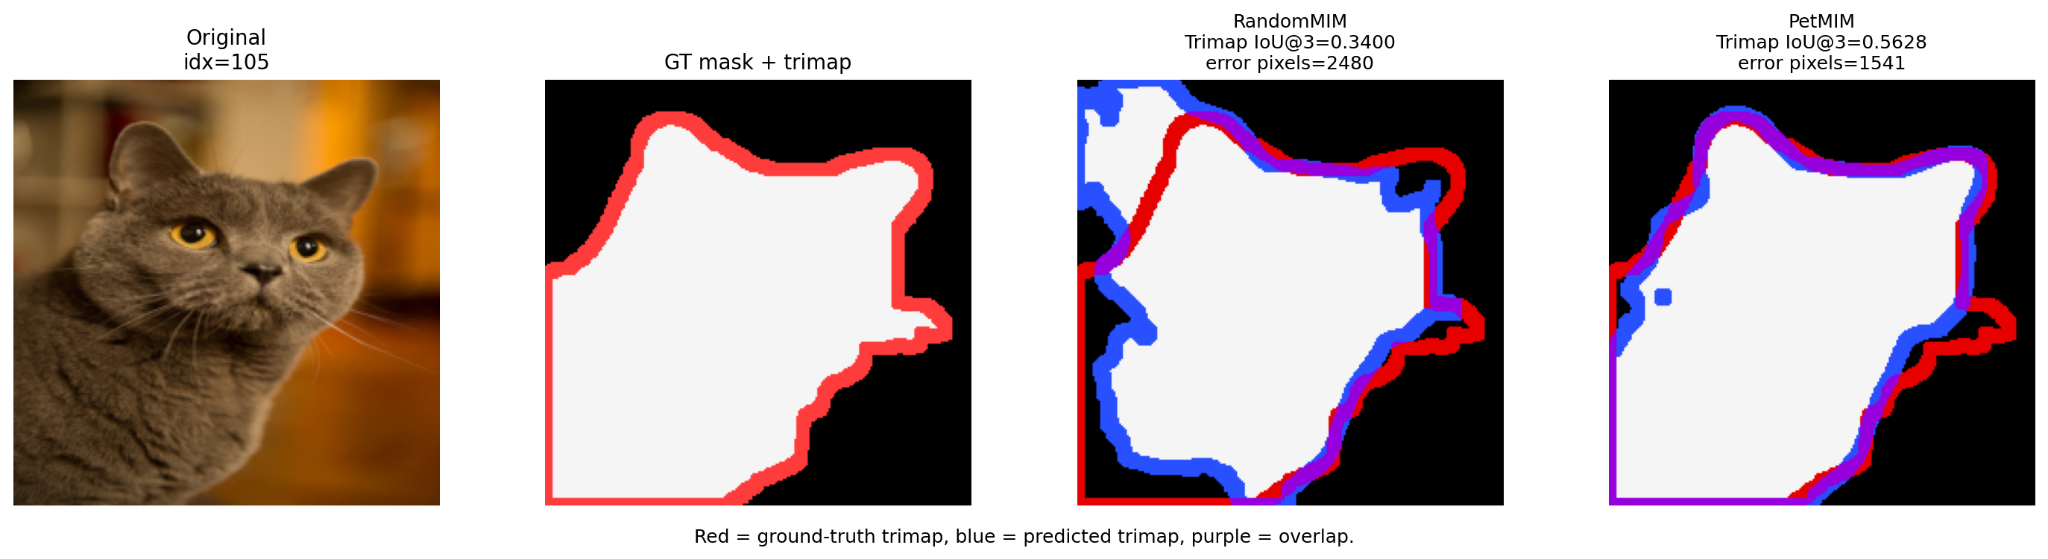
\includegraphics[width=0.98\linewidth]{figures/case_idx105_compare.png}
    \vspace{0.3em}
    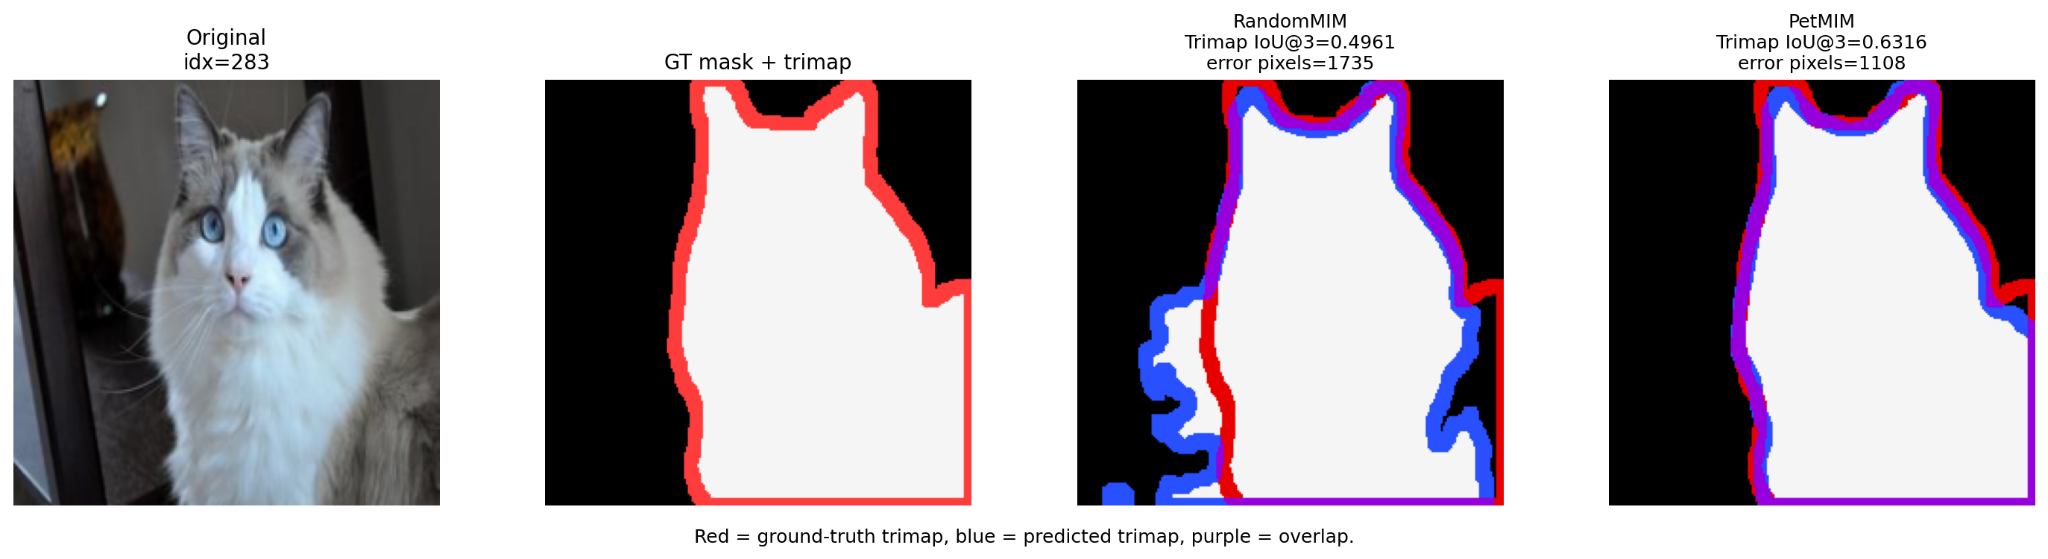
\includegraphics[width=0.98\linewidth]{figures/case_idx283_compare.png}
    \vspace{0.3em}
    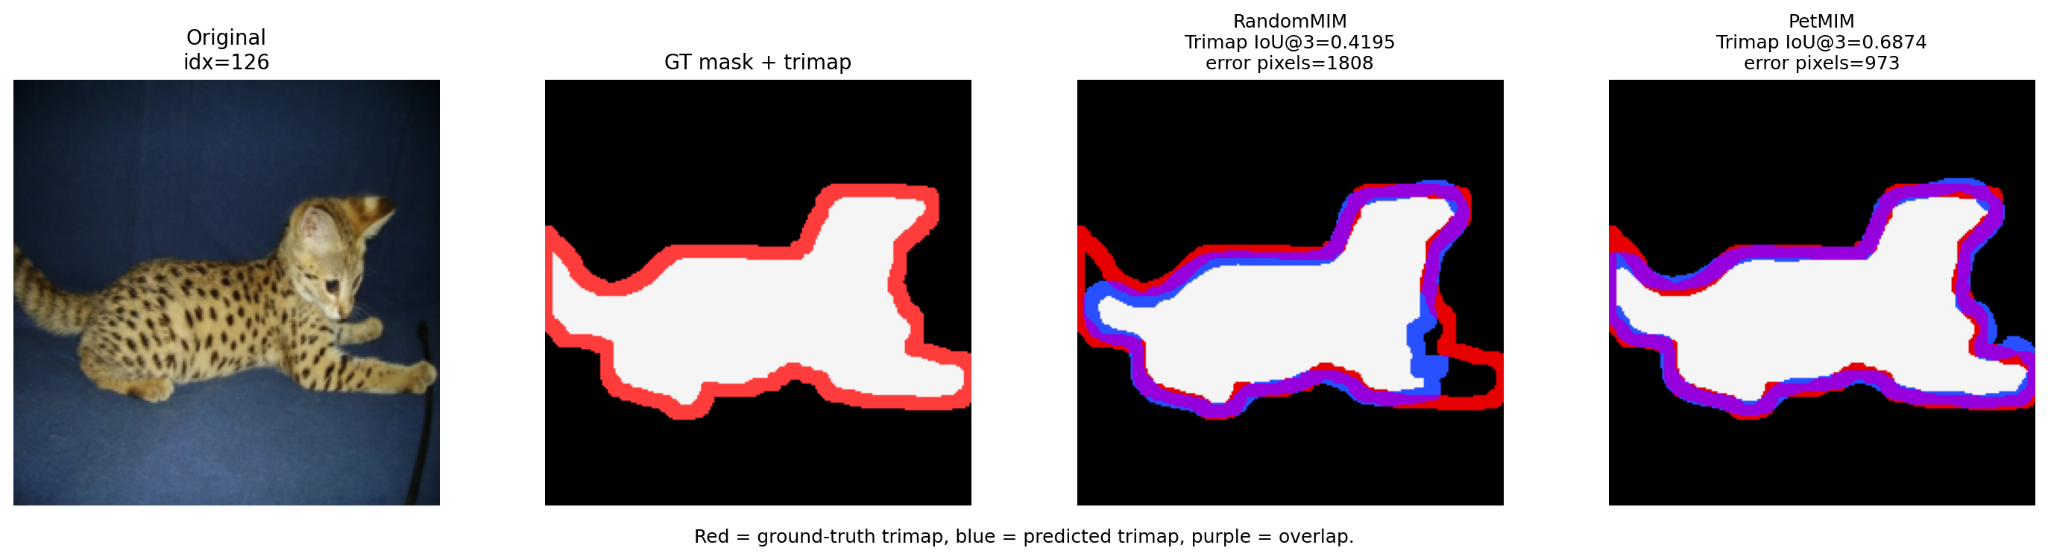
\includegraphics[width=0.98\linewidth]{figures/case_idx126_compare.png}
    \caption{Qualitative comparison between RandomMIM and PetMIM on selected Oxford-IIIT Pet test cases. Each row shows the original image, the ground-truth mask with its trimap band, the RandomMIM trimap overlay, and the PetMIM trimap overlay. Red denotes the ground-truth trimap region, blue denotes the predicted trimap region, and purple denotes their overlap. PetMIM produces boundary regions that better align with the ground-truth trimap and reduces boundary-region error pixels in these examples.}
    \label{fig:qualitative}
\end{figure}

\FloatBarrier

\section{Conclusion}

This paper presents PetMIM, a structure-aware masked image modeling pretraining method for pet image segmentation. PetMIM computes patch-level structure scores from edge, texture, and low-color-contrast information, then applies a 75\% structure-guided and 25\% random mixed masking strategy. The pretrained ResNet18 encoder is transferred to a fixed ResNet18-U-Net segmentation model. On the Oxford-IIIT Pet benchmark, PetMIM outperforms Scratch and RandomMIM across global overlap, spatial distance, Boundary F1, and trimap metrics. Hard-case analysis further shows that PetMIM is especially effective for boundary-complex and low-contrast pet images.

The current paper still has limitations. First, the results are based on one main training protocol and should be strengthened with multi-seed experiments. Second, the structure score is hand-designed; stronger priors, learned saliency, or foundation-model features such as DINO~\cite{caron2021emerging} may provide better task-adaptive masking in future work. AI tools were used to assist with paper organization, language polishing, LaTeX formatting, and code debugging. All experiments, result values, and analyses reported in this paper were conducted and verified by the authors.

\begin{thebibliography}{99}

\bibitem{parkhi2012cats}
O. M. Parkhi, A. Vedaldi, A. Zisserman, and C. V. Jawahar.
\newblock Cats and dogs.
\newblock In \emph{IEEE Conference on Computer Vision and Pattern Recognition}, pages 3498--3505, 2012.

\bibitem{everingham2010pascal}
M. Everingham, L. Van Gool, C. K. I. Williams, J. Winn, and A. Zisserman.
\newblock The Pascal visual object classes (VOC) challenge.
\newblock \emph{International Journal of Computer Vision}, 88(2):303--338, 2010.

\bibitem{lin2014microsoft}
T.-Y. Lin, M. Maire, S. Belongie, J. Hays, P. Perona, D. Ramanan, P. Doll{\'a}r, and C. L. Zitnick.
\newblock Microsoft COCO: Common objects in context.
\newblock In \emph{European Conference on Computer Vision}, pages 740--755, 2014.


\bibitem{he2016deep}
K. He, X. Zhang, S. Ren, and J. Sun.
\newblock Deep residual learning for image recognition.
\newblock In \emph{IEEE Conference on Computer Vision and Pattern Recognition}, pages 770--778, 2016.

\bibitem{long2015fully}
J. Long, E. Shelhamer, and T. Darrell.
\newblock Fully convolutional networks for semantic segmentation.
\newblock In \emph{IEEE Conference on Computer Vision and Pattern Recognition}, pages 3431--3440, 2015.

\bibitem{ronneberger2015unet}
O. Ronneberger, P. Fischer, and T. Brox.
\newblock U-Net: Convolutional networks for biomedical image segmentation.
\newblock In \emph{Medical Image Computing and Computer-Assisted Intervention}, pages 234--241, 2015.

\bibitem{chen2018encoder}
L.-C. Chen, Y. Zhu, G. Papandreou, F. Schroff, and H. Adam.
\newblock Encoder-decoder with atrous separable convolution for semantic image segmentation.
\newblock In \emph{European Conference on Computer Vision}, pages 801--818, 2018.

\bibitem{xie2021segformer}
E. Xie, W. Wang, Z. Yu, A. Anandkumar, J. M. Alvarez, and P. Luo.
\newblock SegFormer: Simple and efficient design for semantic segmentation with transformers.
\newblock In \emph{Advances in Neural Information Processing Systems}, volume 34, pages 12077--12090, 2021.

\bibitem{qin2019basnet}
X. Qin, Z. Zhang, C. Huang, M. Dehghan, O. R. Zaiane, and M. Jagersand.
\newblock BASNet: Boundary-aware salient object detection.
\newblock In \emph{IEEE/CVF Conference on Computer Vision and Pattern Recognition}, pages 7479--7489, 2019.

\bibitem{kervadec2019boundary}
H. Kervadec, J. Bouchtiba, C. Desrosiers, E. Granger, J. Dolz, and I. Ben Ayed.
\newblock Boundary loss for highly unbalanced segmentation.
\newblock In \emph{Medical Imaging with Deep Learning}, pages 285--296, 2019.

\bibitem{kirillov2020pointrend}
A. Kirillov, Y. Wu, K. He, and R. Girshick.
\newblock PointRend: Image segmentation as rendering.
\newblock In \emph{IEEE/CVF Conference on Computer Vision and Pattern Recognition}, pages 9799--9808, 2020.

\bibitem{chen2020simclr}
T. Chen, S. Kornblith, M. Norouzi, and G. Hinton.
\newblock A simple framework for contrastive learning of visual representations.
\newblock In \emph{International Conference on Machine Learning}, pages 1597--1607, 2020.

\bibitem{he2020moco}
K. He, H. Fan, Y. Wu, S. Xie, and R. Girshick.
\newblock Momentum contrast for unsupervised visual representation learning.
\newblock In \emph{IEEE/CVF Conference on Computer Vision and Pattern Recognition}, pages 9729--9738, 2020.

\bibitem{grill2020byol}
J.-B. Grill, F. Strub, F. Altch{\'e}, C. Tallec, P. Richemond, E. Buchatskaya, C. Doersch, B. Avila Pires, Z. Guo, M. Azar, B. Piot, K. Kavukcuoglu, R. Munos, and M. Valko.
\newblock Bootstrap your own latent: A new approach to self-supervised learning.
\newblock In \emph{Advances in Neural Information Processing Systems}, volume 33, pages 21271--21284, 2020.

\bibitem{chen2021simsiam}
X. Chen and K. He.
\newblock Exploring simple Siamese representation learning.
\newblock In \emph{IEEE/CVF Conference on Computer Vision and Pattern Recognition}, pages 15750--15758, 2021.

\bibitem{bao2022beit}
H. Bao, L. Dong, and F. Wei.
\newblock BEiT: BERT pre-training of image transformers.
\newblock In \emph{International Conference on Learning Representations}, 2022.

\bibitem{he2022masked}
K. He, X. Chen, S. Xie, Y. Li, P. Doll{\'a}r, and R. Girshick.
\newblock Masked autoencoders are scalable vision learners.
\newblock In \emph{IEEE/CVF Conference on Computer Vision and Pattern Recognition}, pages 16000--16009, 2022.

\bibitem{xie2022simmim}
Z. Xie, Z. Zhang, Y. Cao, Y. Lin, J. Bao, Z. Yao, Q. Dai, and H. Hu.
\newblock SimMIM: A simple framework for masked image modeling.
\newblock In \emph{IEEE/CVF Conference on Computer Vision and Pattern Recognition}, pages 9653--9663, 2022.

\bibitem{wei2022masked}
C. Wei, H. Fan, S. Xie, C.-Y. Wu, A. Yuille, and C. Feichtenhofer.
\newblock Masked feature prediction for self-supervised visual pre-training.
\newblock In \emph{IEEE/CVF Conference on Computer Vision and Pattern Recognition}, pages 14668--14678, 2022.

\bibitem{tian2023spark}
K. Tian, Y. Jiang, Q. Diao, C. Lin, L. Wang, and Z. Yuan.
\newblock Designing BERT for convolutional networks: Sparse and hierarchical masked modeling.
\newblock In \emph{International Conference on Learning Representations}, 2023.

\bibitem{zhang2026orgmim}
Y. Zhang, H. Zhai, J. Guo, Z. Li, J. Liu, and H. Han.
\newblock Masked image modeling for generalizable organelle segmentation in volume EM.
\newblock \emph{IEEE Transactions on Medical Imaging}, 2026.
\newblock doi:10.1109/TMI.2026.3667612.

\bibitem{caron2021emerging}
M. Caron, H. Touvron, I. Misra, H. J{\'e}gou, J. Mairal, P. Bojanowski, and A. Joulin.
\newblock Emerging properties in self-supervised vision transformers.
\newblock In \emph{IEEE/CVF International Conference on Computer Vision}, pages 9650--9660, 2021.

\end{thebibliography}

\end{document}
